%%%%%%%%%%%%%%%%%%%%%%%%%%%%%%%%%%%%%%%%%%  不使用 authblk 包制作标题  %%%%%%%%%%%%%%%%%%%%%%%%%%%%%%%%%%%%%%%%%%%%%%
%-------------------------------PPT Title-------------------------------------
\title{16-磁性与自旋波}
%-----------------------------------------------------------------------------
%----------------------------Author & Date------------------------------------

%\author[\textrm{Jun\_Jiang}]{姜\;\;骏\inst{}} %[]{} (optional, use only with lots of authors)
%% - Give the names in the same order as the appear in the paper.
%% - Use the \inst{?} command only if the authors have different
%%   affiliation.
%\institute[BCC]{\inst{}%
\institute[Gain~Strong]{\inst{}%
%\vskip -20pt 北京市计算中心}
\vskip -20pt {\large 格致斯创~科技}}
\date[\today] % (optional, should be abbreviation of conference name)
{%	{\fontsize{6.2pt}{4.2pt}\selectfont{\textcolor{blue}{E-mail:~}\url{jiangjun@bcc.ac.cn}}}
\vskip 45 pt {\fontsize{8.2pt}{6.2pt}\selectfont{%清华大学\;\;物理系% 报告地点
	\vskip 5 pt \textrm{2023.07.15}}}
}

%% - Either use conference name or its abbreviation
%% - Not really information to the audience, more for people (including
%%   yourself) who are reading the slides onlin%%   yourself) who are reading the slides onlin%%   yourself) who are reading the slides onlineee
%%%%%%%%%%%%%%%%%%%%%%%%%%%%%%%%%%%%%%%%%%%%%%%%%%%%%%%%%%%%%%%%%%%%%%%%%%%%%%%%%%%%%%%%%%%%%%%%%%%%%%%%%%%%%%%%%%%%%

\subject{}
% This is only inserted into the PDF information catalog. Can be left
% out.
%\maketitle
\frame
{
%	\frametitle{\fontsize{9.5pt}{5.2pt}\selectfont{\textcolor{orange}{“高通量并发式材料计算算法与软件”年度检查}}}
\titlepage
}
%-----------------------------------------------------------------------------

%------------------------------------------------------------------------------列出全文 outline ---------------------------------------------------------------------------------
%\section*{}
%\frame[allowframebreaks]
%{
%  \frametitle{Outline}
%%  \frametitle{\textcolor{mycolor}{\secname}}
%  \tableofcontents%[current,currentsection,currentsubsection]
%}
%%在每个section之前列出全部Outline
%%类似的在每个subsection之前列出全部Outline是\AtBeginSubsection[]
%\AtBeginSection[]
%{
%  \frame<handout:0>%[allowframebreaks]
%  {
%    \frametitle{Outline}
%%全部Outline中,本部分加亮
%    \tableofcontents[current,currentsection]
%  }
%}

%-----------------------------------------------PPT main Body------------------------------------------------------------------------------------
\small
%\section{\rm{VASP~}软件中\rm{PAW~}计算的实现}
%\frame
%
%	\frametitle{\textrm{VASP}计算的特色}
%	相比于与普通的第一原理计算软件,\textrm{VASP}很好地平衡了计算效率和精度的问题,总的来说,\textrm{VASP}主要通过这几个特色保证了计算的高效能
%	\begin{itemize}
%	     \item 迭代与优化算法的多样性\\
%		     本质上电荷密度迭代 \textrm{\&\&} 体系总能量优化是相同的优化问题,采用了类似的算法\upcite{CMS6-15_1996,PRB54-11169_1996}:\\
%			\textcolor{blue}{\textrm{Pseudo-Newton、Conjugate-Gradient、Broyden~mix、damping-factor、RMM-DIIS}}
%	     \item 尽可能采用局域基(原子轨道基)函数:~\\
%		     \textcolor{blue}{\textrm{LREAL}}=\textcolor{red}{\textrm{.TRUE.}}\\
%			优化的投影函数也尽可能在实空间表示
%	     \item \textrm{PAW}原子数据集:\textcolor{blue}{优异的赝势}\upcite{PRB59-1758_1999}
%	\end{itemize}
%}
\section{磁性与自旋波}
\frame
{
	\frametitle{电子的本征属性:~自旋}
\begin{figure}[h!]
\vspace*{-0.08in}
\centering
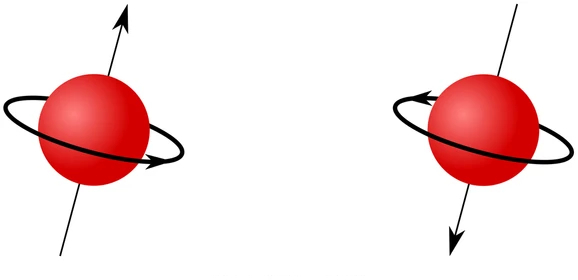
\includegraphics[height=2.05in,width=4.00in,viewport=0 0 580 290,clip]{Figures/electron-spin_2.jpeg}
\caption{\tiny \textrm{Electron spin is a fundamental property of electrons.}}%(与文献\cite{EPJB33-47_2003}图1对比)
\label{Fig:Electron-spin}
\end{figure}
}

\frame
{
	\frametitle{简单磁结构~\textrm{.VS.}~复杂磁结构}
\begin{figure}[h!]
\vspace*{-0.08in}
\centering
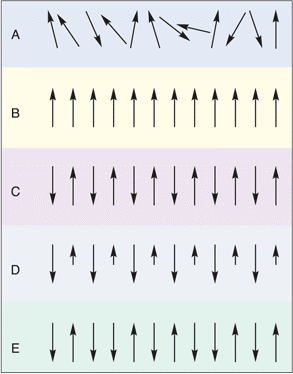
\includegraphics[height=1.05in,width=0.75in]{Figures/Magnet-simple.png}
\caption{\tiny \textrm{Simple Magnetic structure:~Ferromagnetism, Anti-Ferromagnetism, Ferrimagnetism}}%(与文献\cite{EPJB33-47_2003}图1对比)
\label{Fig:Simple-Magnet}
\end{figure}
\begin{figure}[h!]
\vspace*{-0.08in}
\centering
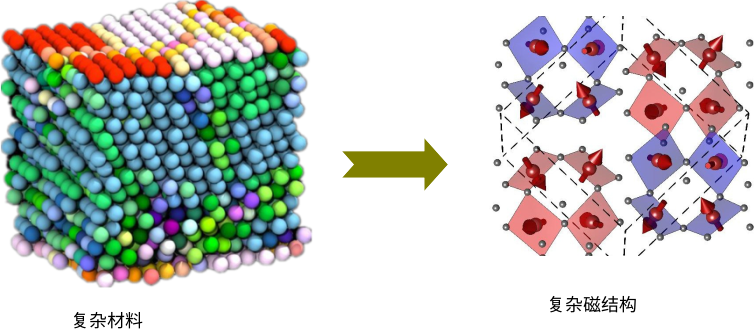
\includegraphics[height=1.05in,width=2.35in]{Figures/Magnet-complex-compound.png}
\hskip 0.5pt
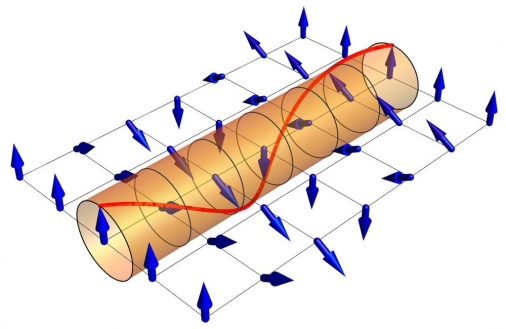
\includegraphics[height=1.05in,width=1.35in]{Figures/Magnet-complex.png}
\caption{\tiny \textrm{Complex Magnetic structure:~Spiral magnet, All-in-all-out, 3k-ordered}}%(与文献\cite{EPJB33-47_2003}图1对比)
\label{Fig:Complex-Magnet}
\end{figure}
}

\frame
{
	\frametitle{电子的自旋与进动}
\begin{figure}[h!]
\vspace*{-0.08in}
\centering
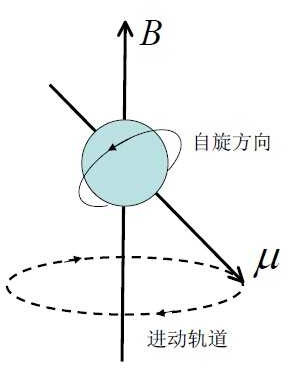
\includegraphics[height=1.95in,width=1.45in,viewport=0 0 210 270,clip]{Figures/Spin_spinor.jpg}
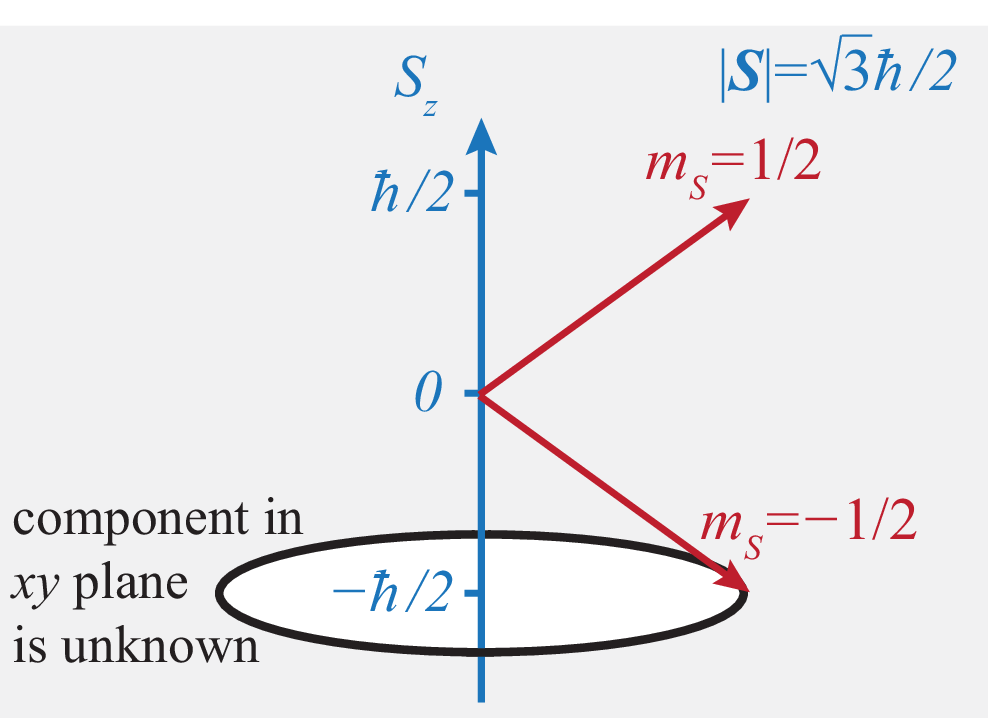
\includegraphics[height=1.95in,width=2.50in,viewport=0 0 580 415,clip]{Figures/Quantization-electron-spin.png}
\caption{\tiny \textrm{Quantisation of electron spin.}}%(与文献\cite{EPJB33-47_2003}图1对比)
\label{Fig:Electron-spin-spinor}
\end{figure}
\textcolor{blue}{磁相互作用比电相互作用弱1$\sim$2个数量级}
}

\frame
{
	\frametitle{自旋极化与磁振子}
	\begin{itemize}
		\item 凝聚态物质中,体系磁性态表现为长程的自旋磁矩有序状态
			\begin{enumerate}
				\item 由于电子-电子相互作用引起的原子局域磁矩(\textcolor{red}{自旋极化})
			\end{enumerate}
	\end{itemize}
		考虑自旋极化,单电子\textrm{Hamiltonian~}可写成二维矩阵
			\begin{displaymath}
				\hspace*{-10pt}\hat H=-\frac12\nabla^2+\sum_{jn}V_{\mathrm C}(|\vec r-\vec t_n-\vec a_j|)\mathbf{I}+\sum_{jn}U^{jn}\hat{V}_{\mathrm{ex}}(|\vec r-\vec t_n-\vec a_j|)(U^{jn})^{-1}
			\end{displaymath}
			矩阵$\mathbf{I}$是二维的单位矩阵,$V_{\mathrm{C}}\mathbf{I}$表示\textrm{Coulomb~}势\\
			矩阵$\mathbf{U}$表示空间坐标与局域坐标的变换关系,选定$z$-轴平行于磁场方向,用\textrm{Euler~}角表示为
			\begin{displaymath}
				\mathbf{U}=\left(
				\begin{matrix}
					\cos(\frac12\beta)\mathrm{exp}[-\mathrm{i}(\alpha+\gamma)/2] &-\sin(\frac12\beta)\mathrm{exp}[-\mathrm{i}(\alpha-\gamma)/2]\\
					\sin(\frac12\beta)\mathrm{exp}[\mathrm{i}(\alpha-\gamma)/2] &\cos(\frac12\beta)\mathrm{exp}[\mathrm{i}(\alpha+\gamma)/2]
				\end{matrix}\right)
			\end{displaymath}
		}

\frame
{
	\frametitle{自旋极化与磁振子}
			局域坐标下,交换势可以表示为
			\begin{displaymath}
				\hat{V}_{\mathrm{ex}}(r)=\left(
				\begin{matrix}
					V_{\mathrm{ex}}^+(r) &0\\
					0 &V_{\mathrm{ex}}^-(r)
				\end{matrix}\right)
			\end{displaymath}
	\begin{itemize}
		\item 局域磁矩间交换作用引起长程磁有序(\textcolor{red}{\textrm{Heisenberg~}}交换)
		\item 除了局域磁矩交换引起的磁有序结构,还有由于能带中巡游电子引起的磁性,称为能带磁性(或巡游电子磁性)
	\end{itemize}
	在能带理论中,磁有序态通过考虑自旋极化,引起\textrm{Hamiltonian~}的改变(\textrm{Zeeman}场强$H_{\mathrm{Zeeman}}$)引入:\\
	自旋极化磁矩$m=n^{\uparrow}-n^{\downarrow}$,引起的势能改变$V_m=\mu H_{\mathrm{Zeeman}}$
	\begin{displaymath}
		\begin{aligned}
			E=&E(V_m)\equiv E_{total}(V_m)\\
			m(\vec r)=&-\frac{\mathrm{d}E}{\mathrm{d}V_m(\vec r)}\\
			\chi(\vec r,\vec r^{\prime})=&-\frac{\mathrm{d}m(\vec r)}{\mathrm{d}V_m(\vec r^{\prime})}=\frac{\mathrm{d}^2E}{\mathrm{d}V_m(\vec r)\mathrm{d}V_m(\vec r^{\prime})}
		\end{aligned}
	\end{displaymath}
}

\frame
{
	\frametitle{铁磁、反铁磁和亚铁磁}
\begin{figure}[h!]
	\vspace{-0.20in}
\centering
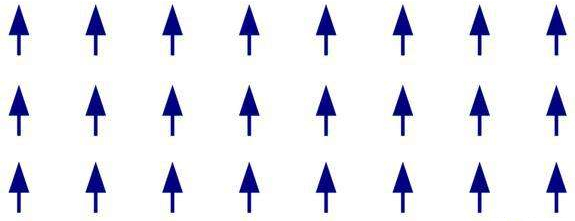
\includegraphics[height=0.95in,width=2.3in,viewport=0 0 350 230,clip]{Figures/Ferromagnetic.jpeg}\\
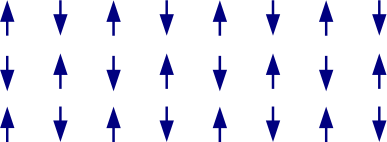
\includegraphics[height=0.85in,width=2.3in,viewport=0 -13 350 155,clip]{Figures/Antiferromagnetic.png}\\
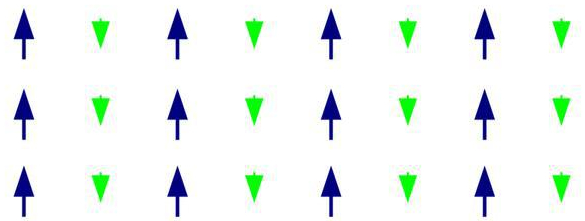
\includegraphics[height=0.88in,width=2.3in,viewport=0 0 350 225,clip]{Figures/Ferrimagnetic.jpeg}
\caption{\tiny \textrm{The model of Ferromagnetic, Antiferromagnetic and Ferrimagnetic.}}%(与文献\cite{EPJB33-47_2003}图1对比)
\label{Ferrimagneitic_Model}
\end{figure} 
}

\frame
{
	\frametitle{\textrm{Heisenberg~}交换模型}
\begin{figure}[h!]
%	\vspace{-0.10in}
\centering
%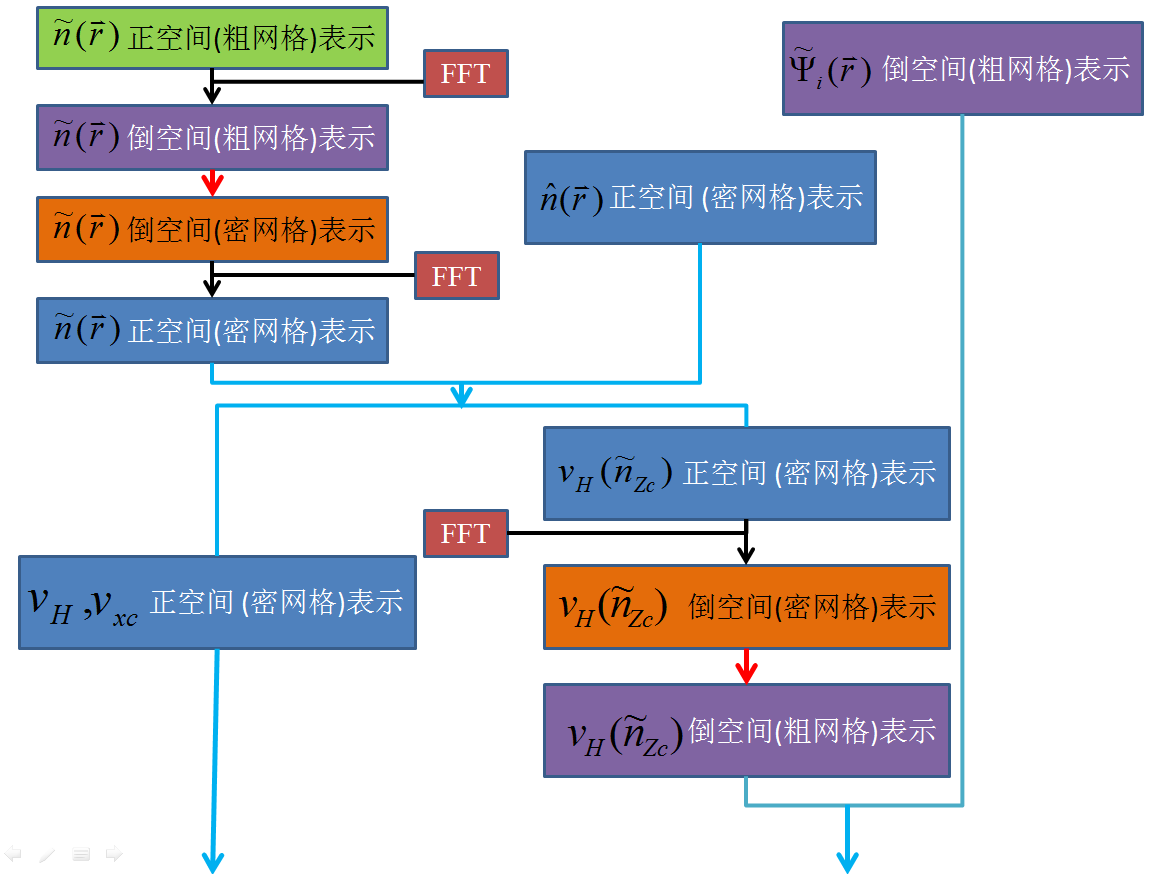
\includegraphics[height=2.7in,width=4.0in,viewport=0 0 1180 875,clip]{Figures/dual_grid.png}
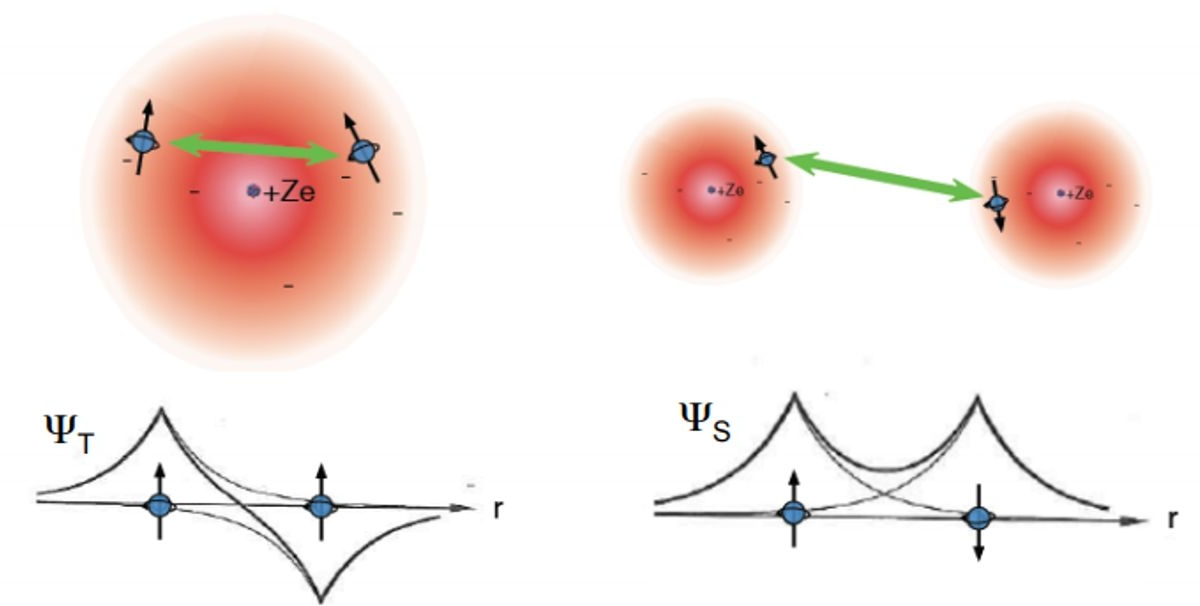
\includegraphics[height=2.0in,width=4.0in,viewport=0 0 580 290,clip]{Figures/Heisenberg_model.jpg}
\caption{\tiny \textrm{The model of Heisenberg-exchange coupling.}}%(与文献\cite{EPJB33-47_2003}图1对比)
\label{Heisenberg_Model}
\end{figure} 
}

\frame
{
	\frametitle{磁振子与自旋响应函数}
	\begin{itemize}
		\item 如果不考虑电子间相互作用,$E-\chi$曲线在净磁矩为0时有极小值,对应于自旋成对(抗磁态)
		\item 考虑电子交换作用,自旋有序(磁性态)能量更有利,因此$V_m(\vec r)$将依赖于$m(\vec r^{\prime})$:\\
			\begin{enumerate}
				\item 如果基态对应$\bar m>0$,则为铁磁态
				\item 如果基态对应$\bar m=0$,则为反铁磁态
			\end{enumerate}
		\item 平均场理论下,磁化率$\chi$即外加磁场的响应函数,\textrm{Stoner~}首先导出磁化率与电子态密度的关系
			\begin{displaymath}
				\chi=\frac{N(0)}{1-IN(0)}
			\end{displaymath}
			其中$N(0)$是\textrm{Fermi~}能级的态密度,磁化有关的有效外势$V_m=V_m^{ext}+Im$
	\end{itemize}
}

\frame
{
	\frametitle{双交换和超交换模型}
\begin{figure}[h!]
	\vspace{-0.35in}
\centering
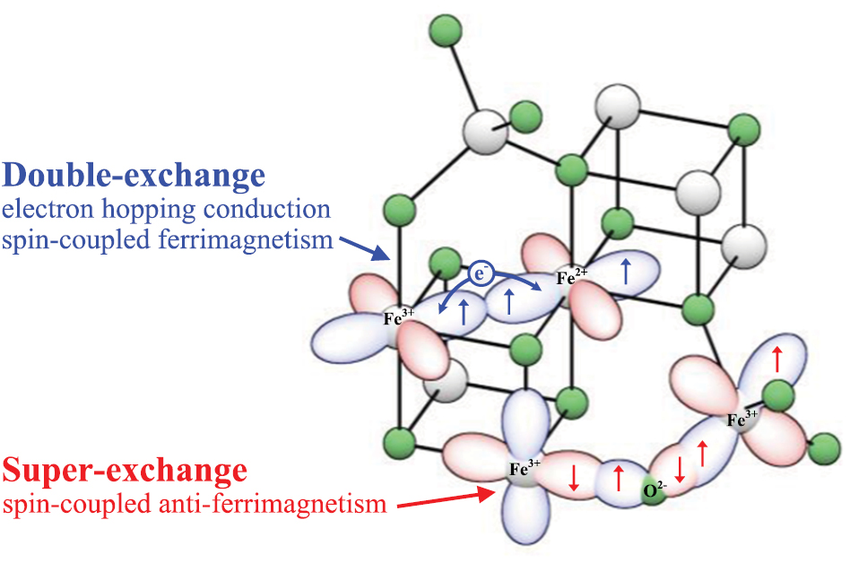
\includegraphics[height=2.50in,width=4.05in,viewport=0 0 205 140,clip]{Figures/Conceptual-representations-of-double-and-super-exchange-interactions-in-Fe3O4-through-d.png}
\caption{\tiny \textrm{Conceptual representations of double and super exchange interactions in \ch{Fe3O4} through \textit{d} orbitals of \ch{Fe2+} and \ch{Fe3+} cations.}}%(与文献\cite{EPJB33-47_2003}图1对比)
\label{double-super-exchange-1}
\end{figure}
}

\frame
{
	\frametitle{超交换模型}
	体系表现出磁有序时,磁性原子的自旋电子与近邻位点磁性原子的电子存在耦合(交换)作用。对于半导体和绝缘体,一般磁性原子(离子)间被其它原子(配位离子)间隔,自旋电子间很难发生直接耦合。这种情况下自旋电子间的相互作用机理称为超交换作用\textrm{(semi-covalent super-exchange interaction)}
\begin{figure}[h!]
	\vspace{-3.5pt}
\centering
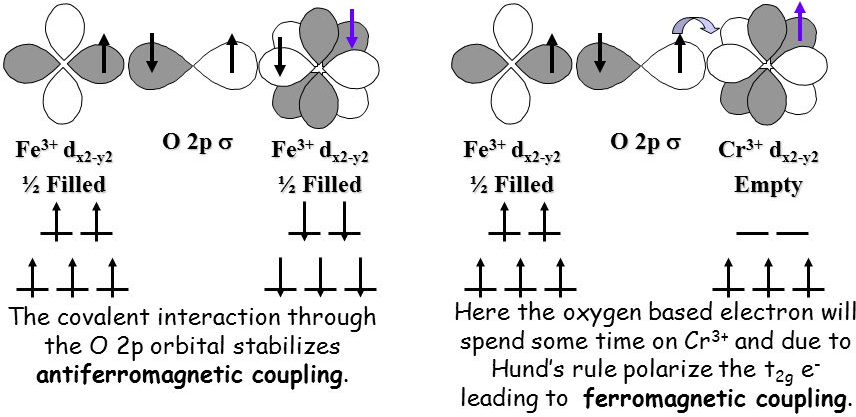
\includegraphics[height=1.80in,width=3.85in,viewport=0 0 660 320,clip]{Figures/Super-exchange-model.jpg}
%\caption{\tiny \textrm{Conceptual representations of double and super exchange interactions in \ch{Fe3O4} through \textit{d} orbitals of \ch{Fe2+} and \ch{Fe3+} cations.}}%(与文献\cite{EPJB33-47_2003}图1对比)
\label{super-exchange-O}
\end{figure}
}

\frame
{
	\frametitle{双交换\textrm{vs.}超交换模型}
\begin{figure}[h!]
	\vspace{-0.15in}
\centering
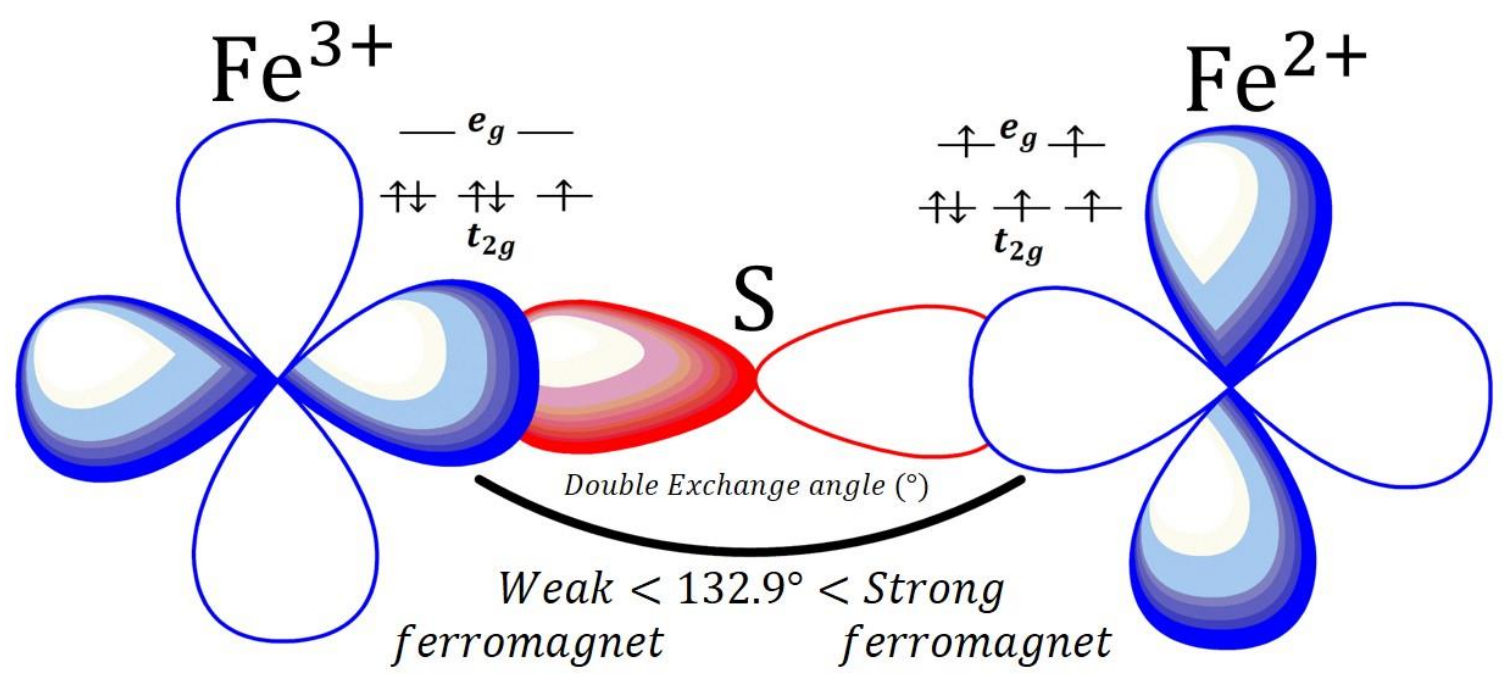
\includegraphics[height=1.70in,width=3.45in,viewport=0 0 1500 700,clip]{Figures/Double-exchange-model.jpg}
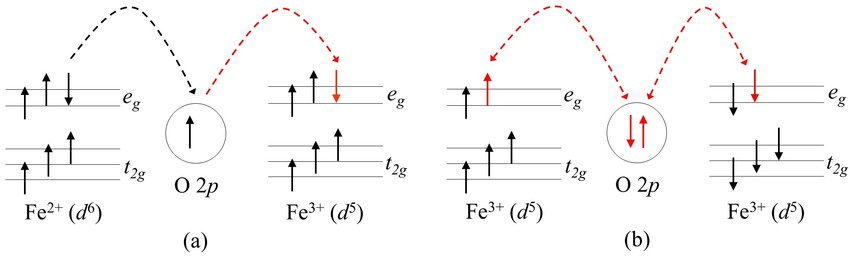
\includegraphics[height=0.90in,width=3.45in,viewport=0 0 640 200,clip]{Figures/Illustration-of-double-exchange-and-superexchange-interactions-in-Fe-3-O-4.jpg}
\caption{\tiny \textrm{Illustration of double exchange (a) and super-exchange interactions in \ch{Fe3O4}.}}%(与文献\cite{EPJB33-47_2003}图1对比)
\label{double-super-exchange-2}
\end{figure}
}

\frame
{
	\frametitle{\textrm{Stoner}模型}
	\begin{itemize}
		\item \textrm{Stoner}将金属的磁性考虑为晶格中巡游的$3d$、$4s$\,电子贡献,其相互作用为$I$,\textrm{Fermi}面附近的\textrm{DOS}为$N(E_{\mathrm F})$
\begin{figure}[h!]
\centering
\vspace*{-0.05in}
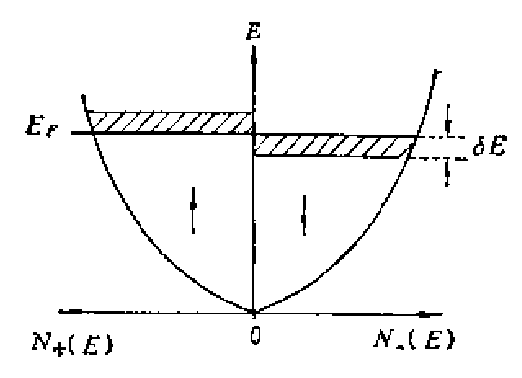
\includegraphics[height=1.0in,width=1.8in,viewport=0 0 800 380,clip]{Figures/Mag_Metal-T0.png}
\caption{\tiny \textrm{The Stoner model.}}%(与文献\cite{EPJB33-47_2003}图1对比)
\label{Mag_Metal-T0}
\end{figure}
		\item 体系的磁性由转变由\textrm{Fermi}面附近能量变化确定
			\begin{displaymath}
				\Delta E=N(E_{\mathrm F})\big[1-IN(E_{\mathrm F})\big](\delta E)^2
			\end{displaymath}
	\end{itemize}
}

\frame
{
	\frametitle{\textrm{Stoner}模型}
	\begin{itemize}
		\item \textrm{Stoner}模型中参数$I$\,主要反应$3d$电子的紧束缚特征,与晶体结构关系不大
		\item \textrm{Stoner}用于孤立原子体系,参数$I$描述自旋电子的裂分,要求:
			\begin{enumerate}
				\item \textcolor{blue}{对\textrm{LSDA}描述的单行列式态,参数$I$可以精确描述原子态的裂分}
				\item \textcolor{blue}{\textrm{LSDA}中应用\textrm{Stoner}模型,参数$I$\,与\textrm{Hubbard}规则的交换参数$U$一致}
			\end{enumerate}
		\item 参数$U$(或$I$~)、$J$的大小\\
			\begin{enumerate}
				\item \textcolor{red}{\textrm{Hund}规则的交换参数$J$的数量级:~ \textrm{1eV}
				\item \textrm{Hubbard}参数$U$的数量级:~\textrm{10eV}}
			\end{enumerate}
	\end{itemize}
}

\frame
{
	\frametitle{能量:~铁磁与反铁磁判据}
\vspace*{-18pt}
\begin{figure}[h!]
\centering
\subfigure[\tiny{\textrm{Structure of Cr}}]{
\label{Fig:WIEN2k_BCC-Cr}
	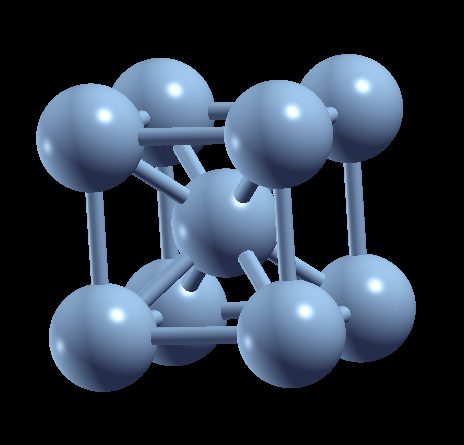
\includegraphics[height=1.20in]{Figures/WIEN2k_BCC_Cr.png}}\\
\subfigure[\tiny{\textrm{Structure of BCC Cr}}]{
\label{Fig:WIEN2k_AFM-Cr-1}
	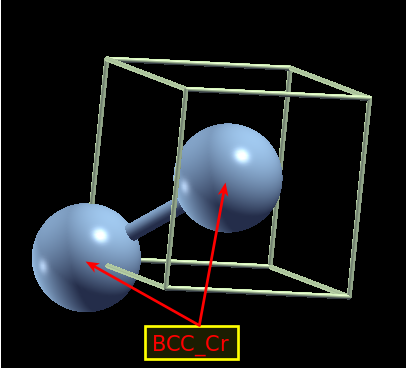
\includegraphics[height=1.20in]{Figures/WIEN2k_BCC_Cr-2.png}}
	\subfigure[\tiny{\textrm{Structure of PCC Cr}}]{
\label{Fig:WIEN2k_AFM-Cr-2}
	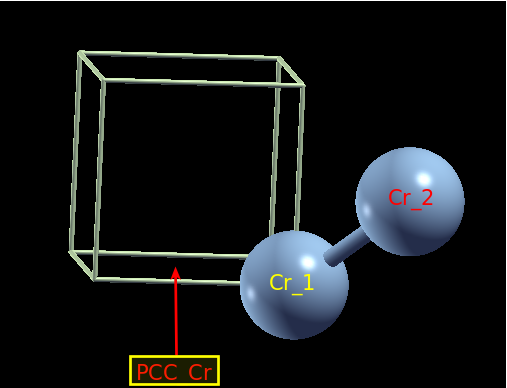
\includegraphics[height=1.20in]{Figures/WIEN2k_AFM_Cr-2.png}}
%\caption{\tiny \textrm{The structure of TiC.}}%(与文献\cite{EPJB33-47_2003}图1对比)
\end{figure}
}

\frame
{
	\frametitle{能量:~铁磁与反铁磁判据}
\vspace*{-8pt}
\begin{figure}[h!]
\centering
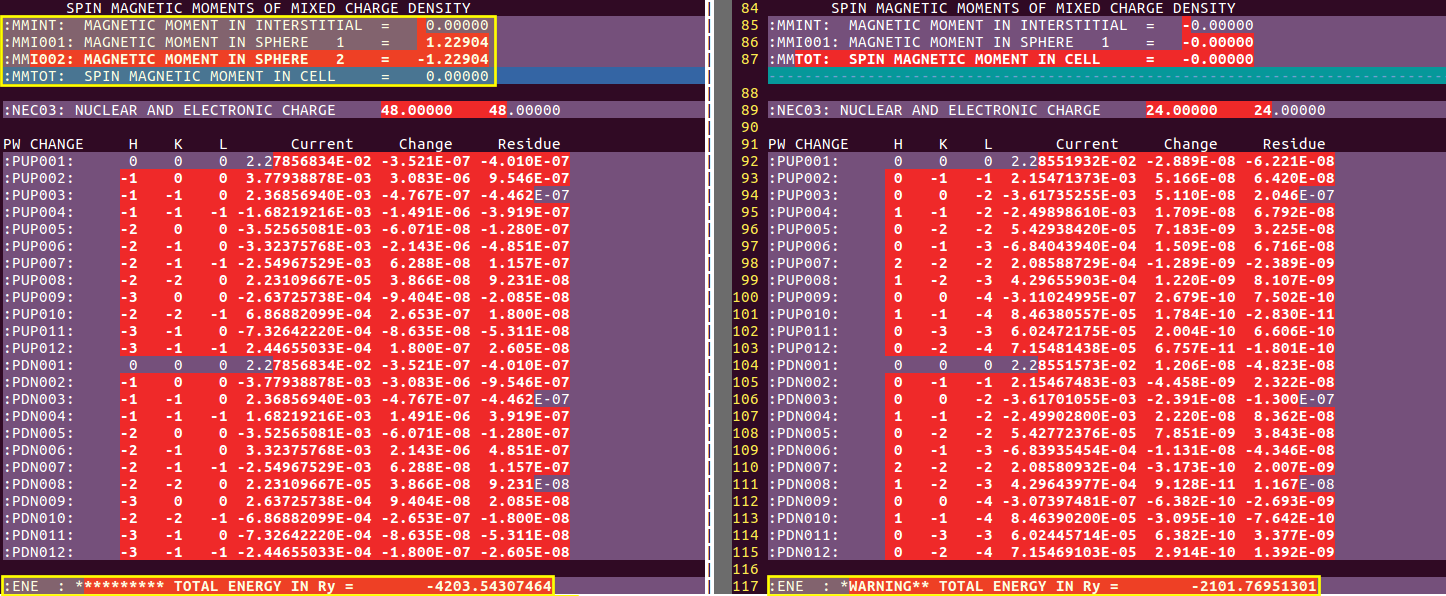
\includegraphics[width=4.1in]{Figures/WIEN2k_AFM_Cr-6.png}
%\caption{\tiny \textrm{The structure of TiC.}}%(与文献\cite{EPJB33-47_2003}图1对比)
\label{Fig:WIEN2k_AFM-Cr-6}
\end{figure}
$E_{\mathrm{AFM}}$:
\begin{displaymath}
	\begin{aligned}
		&-4203.54307464-2\times(-2101.76951301)\\
		=&-0.0405~\mathrm{Ry}\\
		=&-0.11~\mathrm{eV}
	\end{aligned}
\end{displaymath}
}

\frame
{
	\frametitle{自旋波模型}
	\begin{itemize}
		\item 作为平均场近似,分子场理论成功描述了强磁性物质的自发磁化行为,但在低温和\textrm{Curie}温度附近,理论与实验存在明显偏差
		\item 自旋波理论是从体系\textcolor{red}{整体激发}的角度出发,解释自发磁化的低温行为
			\begin{enumerate}
				\item 0\textrm{K~}下电子自旋有序排列(系统基态)
\begin{figure}[h!]
\centering
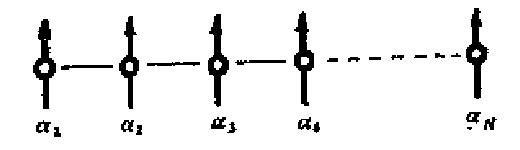
\includegraphics[height=0.50in,width=2.45in,viewport=10 10 600 150,clip]{Figures/Mag_spinwave-0.png}
\caption{\tiny \textrm{The ground state $|0\rangle$.}}%(与文献\cite{EPJB33-47_2003}图1对比)
\label{Mag_spinwave-0}
\end{figure}
				\item 温度略有升高时,电子自旋有一个发生翻转
\begin{figure}[h!]
\centering
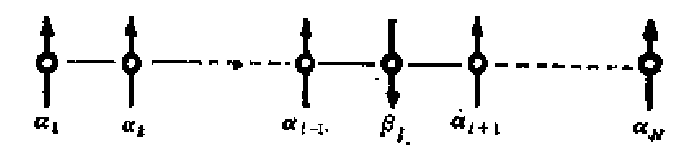
\includegraphics[height=0.50in,width=2.45in,viewport=10 10 680 150,clip]{Figures/Mag_spinwave-1.png}
\caption{\tiny \textrm{The spin flips at $l$:~ $|l\rangle$.}}%(与文献\cite{EPJB33-47_2003}图1对比)
\label{Mag_spinwave-1}
\end{figure}
			\end{enumerate}
	\end{itemize}
}

\frame
{
	\frametitle{自旋波模型}
	某个格点上出现自旋翻转,\textcolor{blue}{由于相邻格点间存在交换作用,使自旋趋于同向排列}
	\begin{itemize}
		\item \textcolor{red}{翻转的自旋将牵动临近格点自旋,使之趋于翻转}
		\item \textcolor{red}{近邻格点自旋力图驱使翻转的自旋重新翻转过来}
	\end{itemize}
	自旋的翻转不会停留在一个格点,而是以波的形式向周围传播:\\
	\textcolor{blue}{这种自旋翻转在晶体中的传播称为}\textcolor{red}{自旋波(又称磁激子)}
\begin{figure}[h!]
\centering
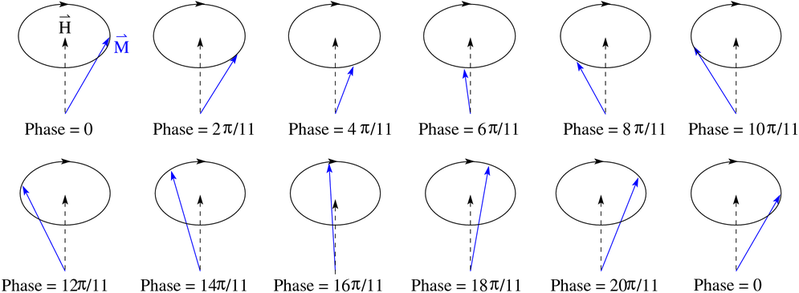
\includegraphics[height=1.15in,width=3.45in,viewport=0 0 830 300,clip]{Figures/Mag_spinwave-2.png}
\caption{\tiny \textrm{The schematic spin-wave.}}%(与文献\cite{EPJB33-47_2003}图1对比)
\label{Mag_spinwave-2}
\end{figure}
}

\frame
{
	\frametitle{非共线磁矩}
	\begin{itemize}
		\item 真实的物理体系中总会出现非共线的磁结构:\\\textcolor{blue}{特别是在铁磁/非磁金属界面上,铁磁性原子磁矩有可能形成非共线排列}
		\item 非共线体系中出现的新现象:\textcolor{blue}{电流诱导的自旋转矩}\\
			\textcolor{red}{非共线的原子磁矩与电子的自旋之间能够通过交换作用,进而引起电子在输运过程中发生自旋翻转,使得自旋向上和自旋向下的输运通道发生了混合}%,并且处在超导态的非磁金属还能够在铁磁体一侧诱导出长程的自旋三重态配对超导性}
		\item 由于非共线磁结构的引入使得问题变得复杂,目前的实验和理论还并不完备
	\end{itemize}
\begin{figure}[h!]
\centering
\vspace*{-0.10in}
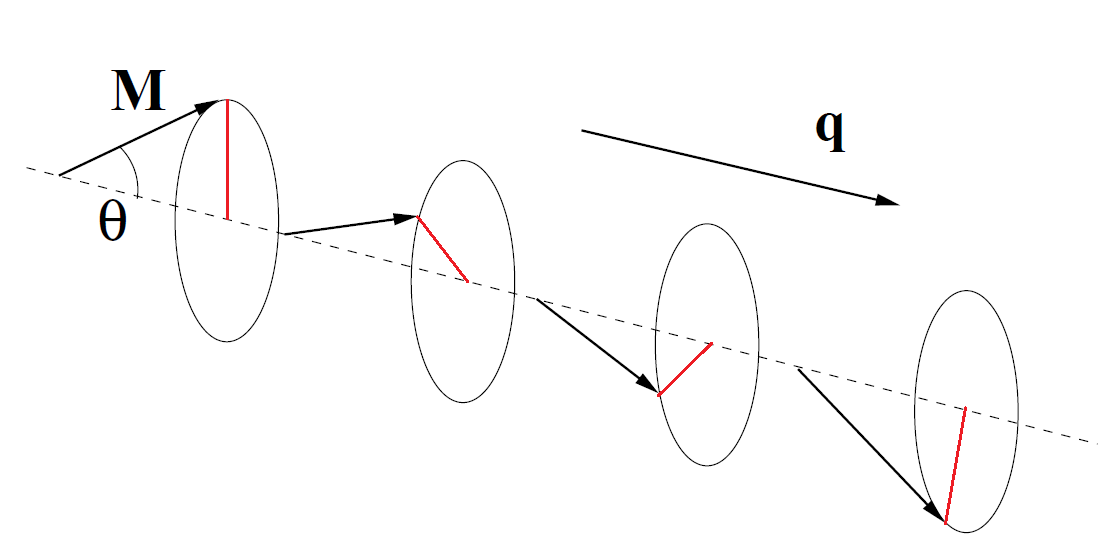
\includegraphics[height=1.05in,width=2.40in,viewport=10 10 840 370,clip]{Figures/Magnet_spinal_wave.png}
\caption{\tiny \textrm{The spiral magnetic structure.}}%(与文献\cite{EPJB33-47_2003}图1对比)
\label{Mag_spinal-wave}
\end{figure}
}

\frame
{
	\frametitle{\textrm{spin-spirals}}
	如果自旋方向随晶格周期也有周期性变化,这种自旋进动(\textrm{spin-spiral})引起体系具有额外的\textcolor{red}{自旋旋进周期性},因此自旋磁矩可以表示为
	\begin{displaymath}
		\vec m(\vec r+\vec R)=
		\left(\begin{matrix}
			m_x(\vec r)\cos(\vec q\cdot\vec R)-m_y(\vec r)\sin(\vec q\cdot\vec R)\\
			m_x(\vec r)\sin(\vec q\cdot\vec R)+m_y(\vec r)\cos(\vec q\cdot\vec R)\\
			m_z(\vec r)
		\end{matrix}\right)
	\end{displaymath}
	这里\textcolor{blue}{$\vec q$是倒空间中自旋进动的单位平移量},因此\\
	\textcolor{brown}{广义\textrm{Bl\"och}定理},波函数和\textrm{Hamiltonian}满足
	\begin{displaymath}
		\begin{aligned}
		&\left(\begin{matrix}
			\Psi_{\vec k}^{\uparrow}(\vec r)\\
			\Psi_{\vec k}^{\downarrow}(\vec r)
		\end{matrix}\right)=\left(
		\begin{matrix}
			\mathrm{e}^{-\mathrm{i}\vec q\cdot\vec R/2} &0\\
			0 &\mathrm{e}^{+\mathrm{i}\vec q\cdot\vec R/2}
		\end{matrix}\right)\left(
		\begin{matrix}
			\Psi_{\vec k}^{\uparrow}(\vec r-\vec R)\\
			\Psi_{\vec k}^{\downarrow}(\vec r-\vec R)
		\end{matrix}
		\right)\\
		&\left(\begin{matrix}
			H^{\alpha\alpha}(\vec q) &V_{xc}^{\alpha\beta}\\
			V_{xc}^{\beta\beta} &H^{\beta\beta}(\vec q)
		\end{matrix}\right)\rightarrow\left(
		\begin{matrix}
			H^{\alpha\alpha}(\vec q) &V_{xc}^{\alpha\beta}\mathrm{e}^{-\mathrm{i}\vec q\cdot\vec r}\\
			V_{xc}^{\beta\alpha}\mathrm{e}^{+\mathrm{i}\vec q\cdot\vec r} &H^{\beta\beta}(\vec q)
		\end{matrix}\right)
		\end{aligned}
	\end{displaymath}
}

\frame
{
	\frametitle{\textrm{DFT}框架下处理非共线磁矩}
	一般地,磁性体系下的\textrm{DFT~}的\textrm{Hamiltonian}:~
	\begin{displaymath}
		H=-\frac{\hbar^2}{2m}\nabla^2+V_{\mathrm{eff}}+\mu_B\vec\sigma\cdot\vec B_{\mathrm{eff}}
	\end{displaymath}
	这里$\mu_B\vec\sigma\cdot\vec B_{\mathrm{eff}}$表示\textcolor{blue}{自旋与有效磁场的相互作用}\\
	有效势、有效磁场是\underline{\textcolor{red}{外场}}和\underline{\textcolor{red}{交换-相关}势}、\underline{\textcolor{red}{交换-相关}场}之和
	\begin{displaymath}
		\begin{aligned}
			V_{\mathrm{eff}}=&V_{\mathrm{ext}}+V_{H}+V_{xc}\\
			\vec B_{\mathrm{eff}}=&\vec B_{\mathrm{ext}}+\vec B_{xc}
		\end{aligned}
	\end{displaymath}
	在\textrm{LDA}下,$E_{xc}(n,\vec m)=\int n\epsilon_{xc}(n,m)\mathrm{d}^3r$,因此交换-相互势和交换-相关场的表示
	\begin{displaymath}
		\begin{aligned}
			V_{xc}=&\frac{\partial E_{xc}(n,\vec m)}{\partial n}=&\epsilon_{xc}(n,m)+n\frac{\partial\epsilon_{xc}(n,m)}{\partial n}\\
			\vec B_{xc}=&\frac{\partial E_{xc}(n,\vec m)}{\partial\vec m}=&\frac{\partial\epsilon_{xc}(n,m)}{\partial m}\vec m
		\end{aligned}
	\end{displaymath}
}

\frame
{
	\frametitle{\textrm{DFT}框架下处理非共线磁矩}
\begin{itemize}
	\item 对\textrm{共线磁性},取外磁场方向与$\mathit{z}$轴方向一致
\begin{displaymath}
	\vec\sigma\cdot\vec B_{\mathrm{eff}}=\sigma_zB_{\mathrm{eff}}
\end{displaymath}
因为
\begin{displaymath}
	\sigma_z=\left(
	\begin{matrix}
		1 &0\\
		0 &-1
	\end{matrix}\right)
\end{displaymath}
由此可得
		\begin{displaymath}
			\hat V=V_{\mathrm{eff}}\mathbf{I}+B_{\mathrm{eff}}\sigma_z=\left(
			\begin{matrix}
				V_{\mathrm{eff}}+\mu_BB_{\mathrm{eff}} &0\\
				0 &V_{\mathrm{eff}}-\mu_BB_{\mathrm{eff}}
			\end{matrix}\right)
		\end{displaymath}
		这种情况下,\textcolor{red}{忽略旋-轨耦合\textrm{(SOC)},\textrm{spin-up}和\textrm{spin-dn}解耦}
\end{itemize}
}

\frame
{
	\frametitle{\textrm{DFT}框架下处理非共线磁矩}
\begin{itemize}
	\item 对\textrm{非共线磁性},标量点积$\mu_B\vec\sigma\cdot\vec B_{\mathrm{eff}}$必须考虑三个分量的贡献,注意到
\begin{displaymath}
	\sigma_x=\left(
	\begin{matrix}
		0 &1\\
		1 &0
	\end{matrix}\right)\quad
	\sigma_y=\left(
	\begin{matrix}
		0 &-\mathrm{i}\\
		\mathrm{i} &0
	\end{matrix}\right)
\end{displaymath}
由此可得
		\begin{displaymath}
			\hat V=V_{\mathrm{eff}}\mathbf{I}+\mu_BB_{\mathrm{eff}}\cdot\vec\sigma=\left(
			\begin{matrix}
				V_{\mathrm{eff}}+\mu_BB_z &\mu_B(B_x-\mathrm{i}B_y)\\
				\mu_B(B_x+\mathrm{i}B_y) &V_{\mathrm{eff}}-\mu_BB_z
			\end{matrix}\right)
		\end{displaymath}
		这种情况下,非对角元项将\textrm{spin-up}和\textrm{spin-dn}耦合在一起

\end{itemize}
}

\frame
{
	\frametitle{\textrm{VASP~}中一般非共线磁性态的计算}
	\textrm{J. K\"ubler}等指出\upcite{JAP63-3482_1988},根据密度泛函理论,当外势是矩阵元为$w^{\alpha\beta}(\vec r)$的$2\times2$矩阵时,令体系的密度矩阵为$\rho^{\alpha\beta}(\vec r)$,则\\
	\textcolor{blue}{体系的电荷密度可以表示为}
	\begin{displaymath}
		Tr[\rho^{\alpha\beta}(r)]\equiv n_{\mathrm{Tr}}(r)=\sum_{\alpha}n^{\alpha\alpha}(\vec r)
	\end{displaymath}
	因此总能量可以表示为
	
	\begin{displaymath}
		\begin{aligned}
			E[\rho^{\alpha\beta}]=&T_0+\sum_{\alpha\beta}\int w^{\alpha\beta}(\vec r)\rho^{\alpha\beta}(\vec r)\mathrm{d}^3r\\
			+&\iint\frac{n_{\mathrm{Tr}}(\vec r^{\prime})n_{\mathrm{Tr}}(\vec r)}{|\vec r-\vec r^{\prime}|}\mathrm{d}^3r\mathrm{d}^3r^{\prime}+E_{\mathrm{XC}}[\rho^{\alpha\beta}]
		\end{aligned}
	\end{displaymath}
}

\frame
{
	\frametitle{\textrm{VASP~}中一般非共线磁性态的计算}
	\textrm{D. Hobbs~}等\upcite{PRB62-11556_2000}\textcolor{red}{考虑磁化密度的贡献后,将总电荷密度矩阵表示为}
	\begin{displaymath}
		\rho^{\alpha\beta}(\vec r)=\left[n_{\mathrm{Tr}}(\vec r)\delta_{\alpha\beta}+\vec m(\vec r)\vec{\sigma}^{\alpha\beta}\right]/2
	\end{displaymath}
	\textcolor{blue}{磁化密度}的表示为
	\begin{displaymath}
		\vec m(\vec r)=\sum_{\alpha\beta}\rho^{\alpha\beta}(\vec r)\cdot\vec{\sigma}^{\alpha\beta}
	\end{displaymath}
	其中\textrm{Pauli~}自旋矩阵$\vec{\sigma}=(\sigma_x,\sigma_y,\sigma_z)$定义为
	\begin{displaymath}
		\sigma_x=\left( 
		\begin{matrix}
			0 &1\\
			1 &0
		\end{matrix}
		\right)\quad
		\sigma_y=\left( 
		\begin{matrix}
			0 &-\mathrm{i}\\
			\mathrm{i} &0
		\end{matrix}
		\right)\quad
		\sigma_z=\left( 
		\begin{matrix}
			1 &0\\
			0 &-1
		\end{matrix}
		\right)
	\end{displaymath}
	因此在\textrm{DFT}框架下能量密度泛函可以表示为
	\begin{displaymath}
		E=\sum_{\alpha}\sum_{n}f_n\langle\Psi_n^{\alpha}|-\frac12\nabla^2|\Psi_n^{\alpha}\rangle+E_{\mathrm{H}}[\textcolor{blue}{n_{\mathrm{Tr}}}+n_Z]+E_{\mathrm{XC}}[\textcolor{red}{\rho^{\alpha\beta}}]
	\end{displaymath}
}

\frame
{
	\frametitle{\textrm{VASP~}中一般非共线磁性态的计算}
	上述表达式中$f_n$是轨道占据数
	
	$E_{\mathrm{H}}[n_{\mathrm{Tr}}+n_Z]$是静电相互作用
	\begin{displaymath}
		E_{\mathrm{H}}[\textcolor{brown}{\rho}]=\frac12\iint\frac{\textcolor{brown}{\rho(\vec r)\rho(\vec r^{\prime})}}{|\vec r-\vec r^{\prime}|}\mathrm{d}\vec r\mathrm{d}\vec r^{\prime}
	\end{displaymath}
	这里$\textcolor{brown}{\rho}=n_{\mathrm{Tr}}+n_Z$

	在\textrm{LSDA}下,交换-相关能泛函表示为
	\begin{displaymath}
		\begin{aligned}
			E_{\mathrm{XC}}[\textcolor{red}{\rho^{\alpha\beta}}]=&\int\textcolor{blue}{n_{\mathrm{Tr}}(\vec r)}\epsilon_{\mathrm{XC}}[\textcolor{red}{\rho^{\alpha\beta}}]\mathrm{d}\vec r\\
			=&\int\textcolor{blue}{n_{\mathrm{Tr}}(\vec r)}\epsilon_{\mathrm{XC}}[\textcolor{blue}{n_{\mathrm{Tr}}(\vec r)},|\vec m(\vec r)|]\mathrm{d}\vec r
		\end{aligned}
	\end{displaymath}
}

%------------------------------------------------------------------------Reference----------------------------------------------------------------------------------------------
\begin{thebibliography}{99}
\frame[allowframebreaks]
{
\frametitle{主要参考文献}
{\tiny
\bibitem{Dai_Qian}戴道生,钱昆明, {\textit{铁磁学}}(上册),\:科学出版社, 北京, 1998
\bibitem{JAP63-3482_1988}\textrm{J. K\"ubler, K. H. H\"ock and J. Sticht. \textit{J. Appl. Phys.}, \textbf{63} (1988), 3482}
\bibitem{PRB62-11556_2000}\textrm{D. Hobbs, G. Kresse and J. Hafner. \textit{Phys. Rev.} B, \textbf{62} (2000), 11556}
}
\nocite*{}
}
\end{thebibliography}

